\chapter{Implementação da Solução}
\label{sec:4-Implementacao}

Este capítulo aprofunda o processo de desenvolvimento da solução para o problema do projeto em 
análise de acordo com a análise e os princípios de \textit{design} discutidos no capítulo anterior. 
Além disso, é efetuada uma análise cuidada dos resultados obtidos através das decisões anteriores, 
revelando os resultados consequentes e a sua concordância com os objetivos discutidos anteriormente.

\section{Tecnologias Utilizadas}

Durante o desenvolvimento do projeto, foram utilizadas várias tecnologias e ferramentas para a 
implementação da solução. Entre as mais relevantes, destacam-se:

\begin{itemize}
  \item \textbf{Apache Storm \cite{storm}:} \textit{Framework} de processamento de 
    \textit{streaming} em tempo real;
  \item \textbf{Apache Kafka \cite{kafka}:} Plataforma de mensagens distribuída;
  \item \textbf{Apache Zookeeper \cite{zookeeper}:} Serviço de coordenação distribuída;
  \item \textbf{Grafana \cite{grafana}:} Plataforma de análise e visualização de dados;
  \item \textbf{Nimbus \cite{nimbus}:} Servidor centralizado que coordena e distribui as topologias 
    do \textit{Apache Storm};
  \item \textbf{Splunk \cite{splunk}:} Plataforma de análise de eventos e dados;
\end{itemize}

\section{Descrição da implementação}

\todo[inline]{TODO}

\subsection{Scaledown do Cluster}

\begin{figure}[H]
  \centerline{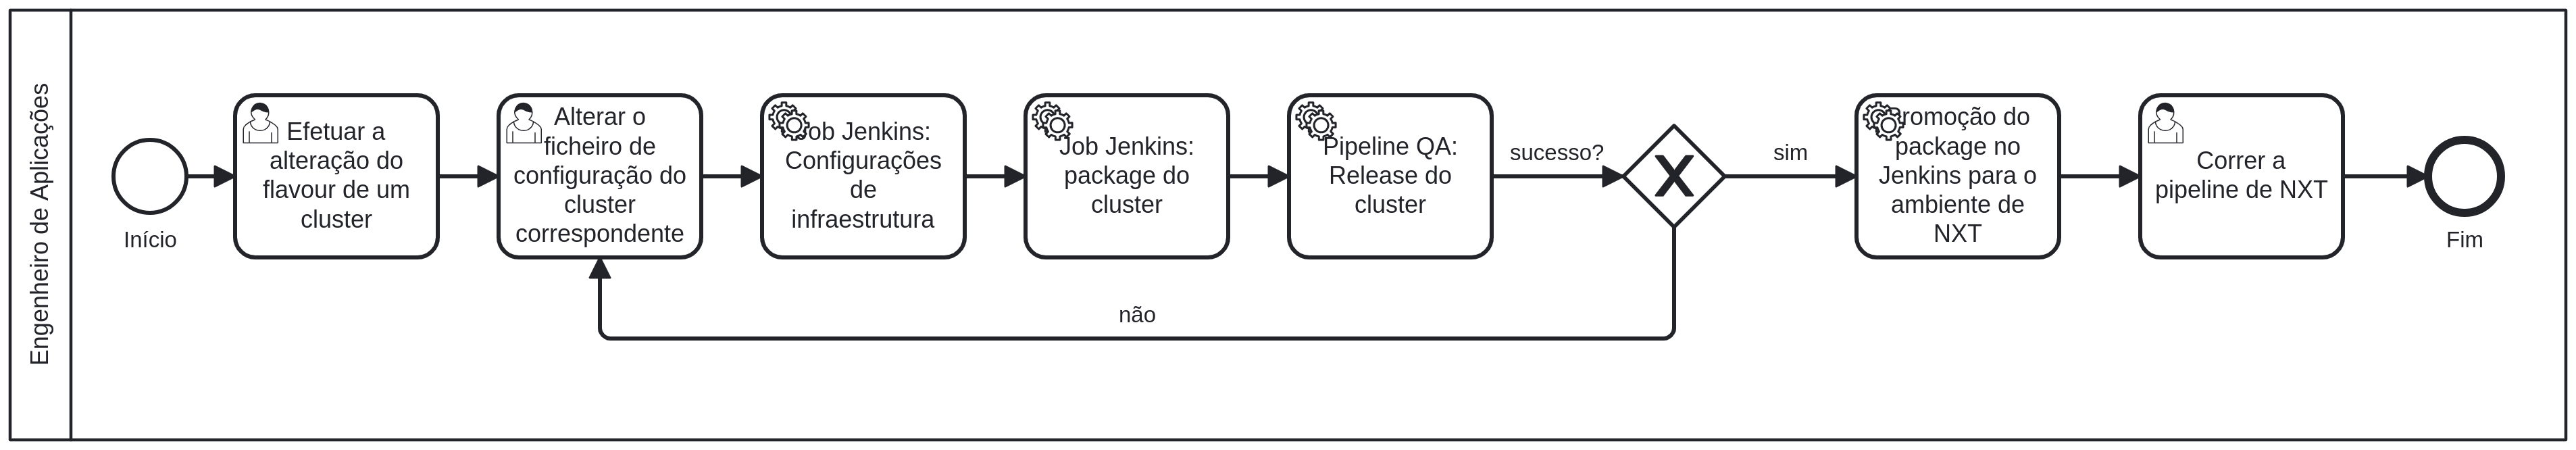
\includegraphics[scale=0.12]{media/content/impl/scaledown_nxt.png}}
  \caption{Processo de \textit{scaledown} de um \textit{cluster} no ambiente de NXT}
  \label{scaledown-nxt}
\end{figure}

\todo[inline]{Incluir BPMNs dos processos de pipelines para alterações de flavours + rollback}

\todo[inline]{Incluir BPMNs do processo de criação de novos clusters (simplificado}

\section{Testes}

\todo[inline]{TODO}

\section{Avaliação da Solução}

\todo[inline]{TODO}

